\documentclass{article}
\usepackage{graphicx} % new way of doing eps files
\usepackage{listings} % nice code layout
\usepackage[usenames]{color} % color
\definecolor{listinggray}{gray}{0.9}
\definecolor{graphgray}{gray}{0.7}
\definecolor{ans}{rgb}{1,0,0}
\definecolor{blue}{rgb}{0,0,1}
% \Verilog{title}{label}{file}
\newcommand{\Verilog}[3]{
  \lstset{language=Verilog}
  \lstset{backgroundcolor=\color{listinggray},rulecolor=\color{blue}}
  \lstset{linewidth=\textwidth}
  \lstset{commentstyle=\textit, stringstyle=\upshape,showspaces=false}
  \lstset{frame=tb}
  \lstinputlisting[caption={#1},label={#2}]{#3}
}


\author{Cameron Anderson}
\title{Class Report 1: Reaction Timer}

\begin{document}
\maketitle

\section{Introduction}
The goal of this assignment is to use Vivado Design Suite to program the Nexys 4 DDR board to create a reaction timer that displays in milliseconds on the seven-segment display how long it takes for a user to press a button after noticing a visual stimulus, in this case a lit LED. Additionally, the assignment should be able to be reset after each use and tell when the user has cheated by pressing the button before the visual stimulus has appeared. 

\section{Experimental Plan}
As seen in Figure~\ref{fig:TimerStateMachine} on page~\pageref{fig:TimerStateMachine}, the project needs a finite state machine to transition the different states of interaction with the device. Additionally, a clock divider is needed to return values in milliseconds to the user. This particular clock divider also features the state machine shown in Figure~\ref{fig:ClockDividerStateMachine} on page~\pageref{fig:ClockDividerStateMachine} that loads a register with the predetermined value and counts down until half of a millisecond has passed. The clock divider then changes the millisecond clock output. To keep users from anticipating when the LED will light, a pseudorandom number generator is incorporated into the project. The LSFR module outputs a single random bit that is shifted each clock cycle into the counter register in the top module that determines the length of wait time until the LED lights. Two additional modules to drive the seven-segment display and to convert hexidecimal to seven-segment values are also required for this project. 

\begin{figure} [h]
\begin{center}
\caption{Main State Machine}\label{fig:TimerStateMachine}
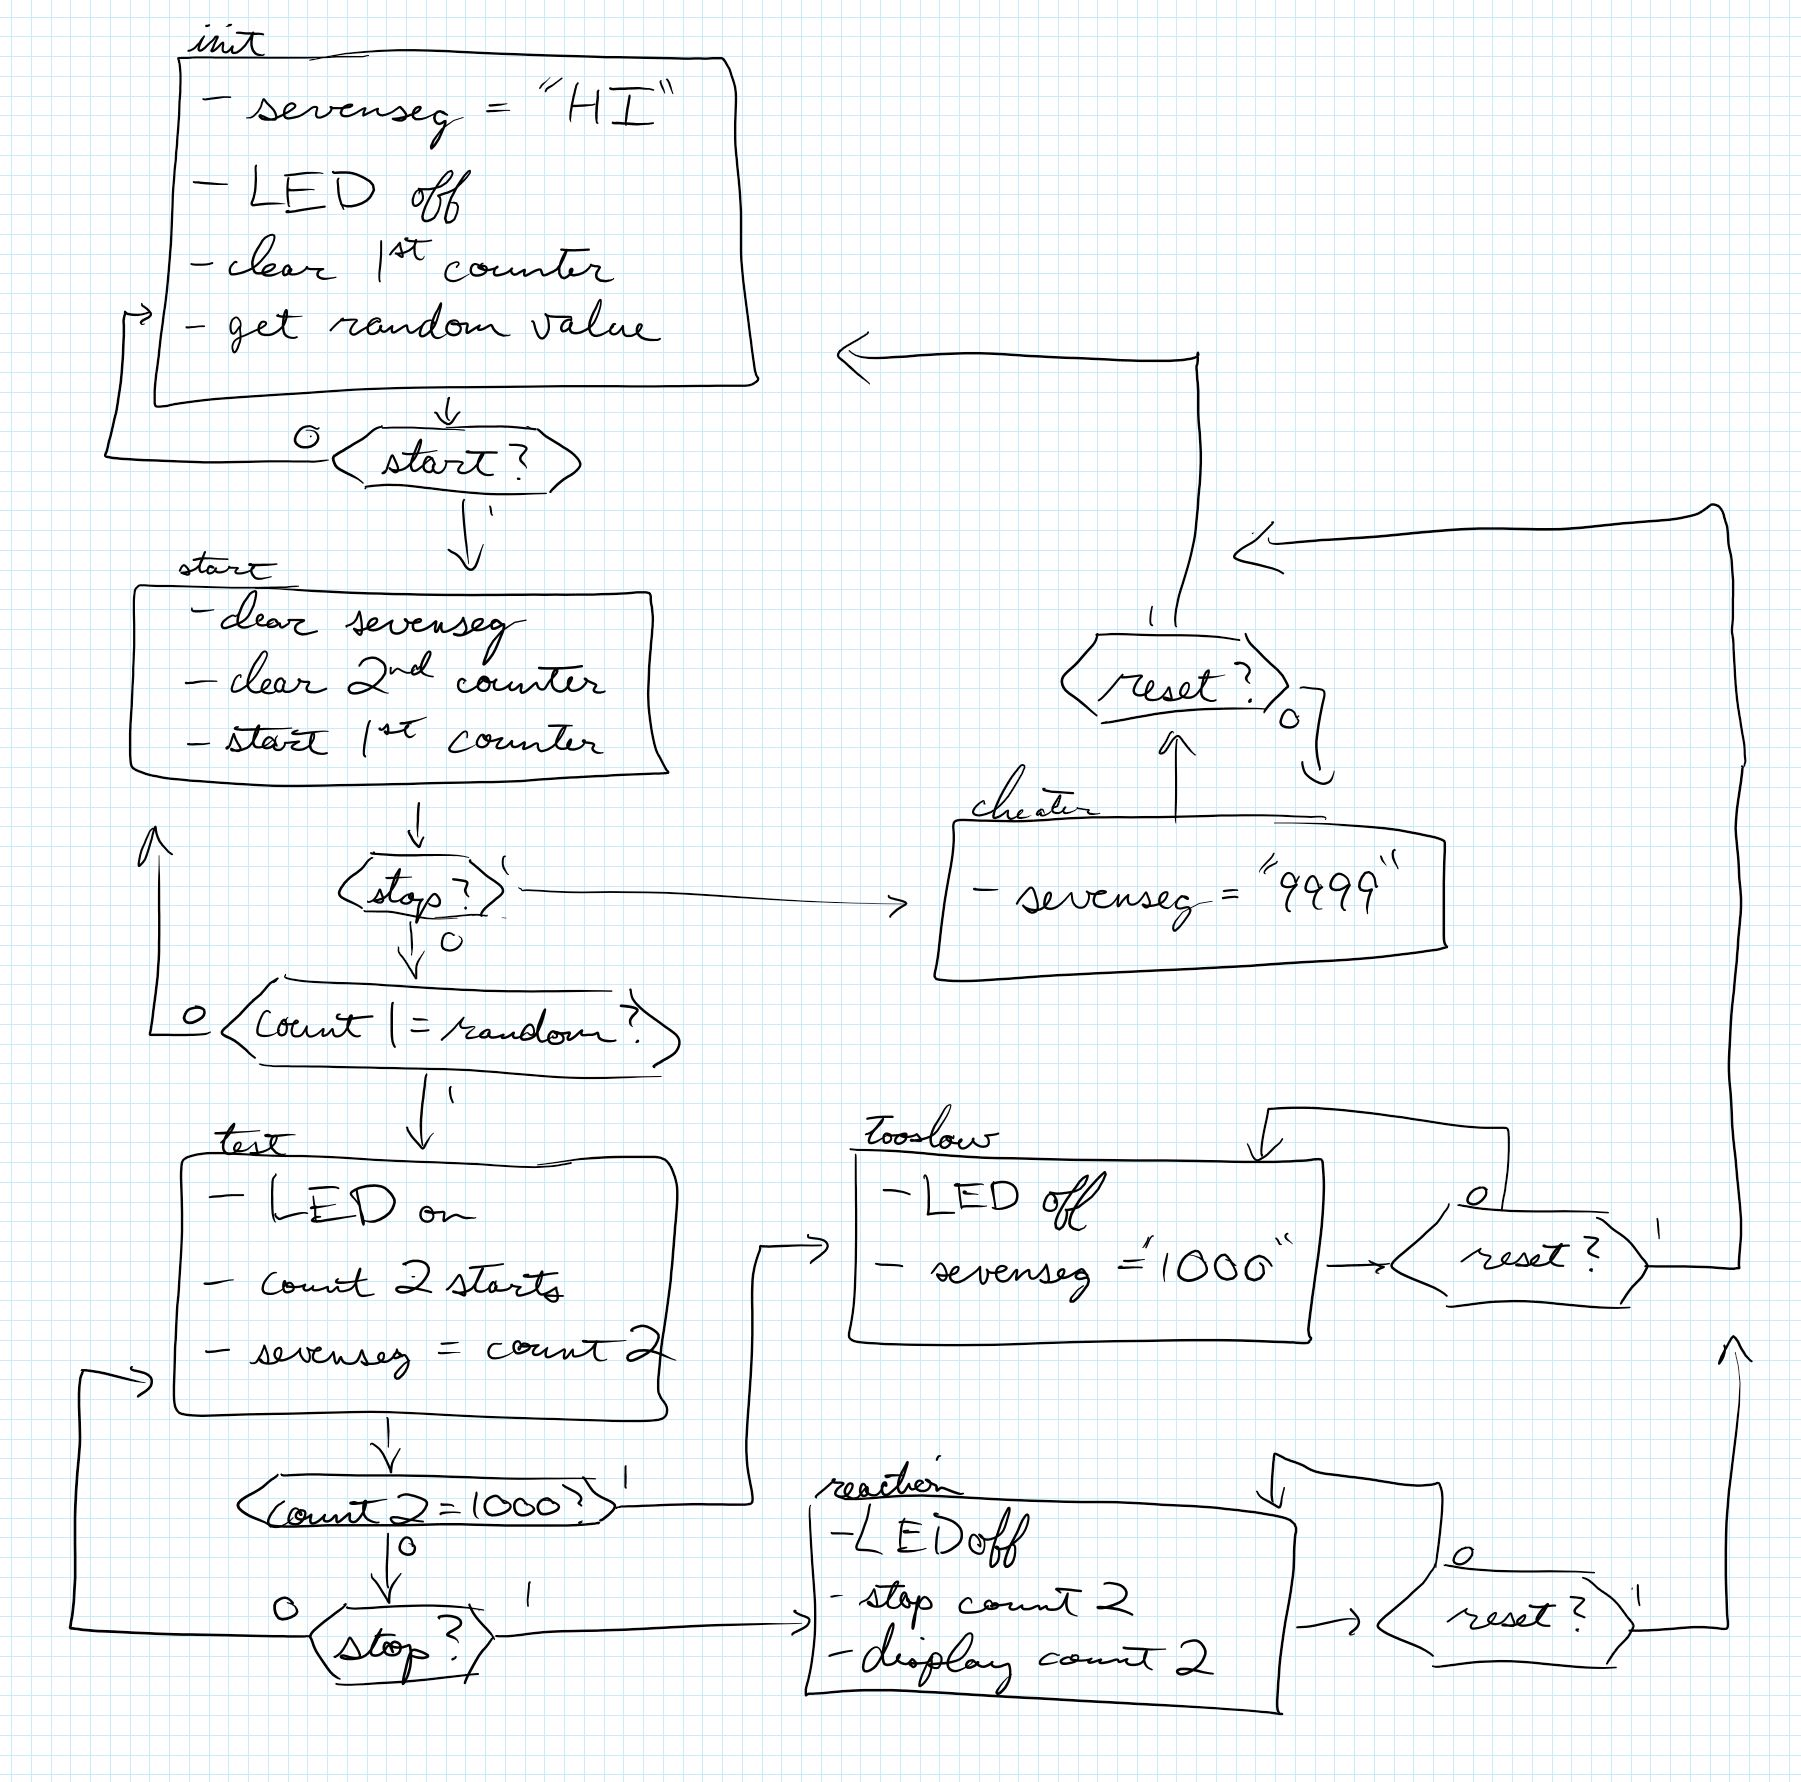
\includegraphics[width=0.9\textwidth]{TimerStateMachine.jpg}
\end{center}
\end{figure}

\begin{figure} [h]
\begin{center}
\caption{Clock Divider State Machine}\label{fig:ClockDividerStateMachine}
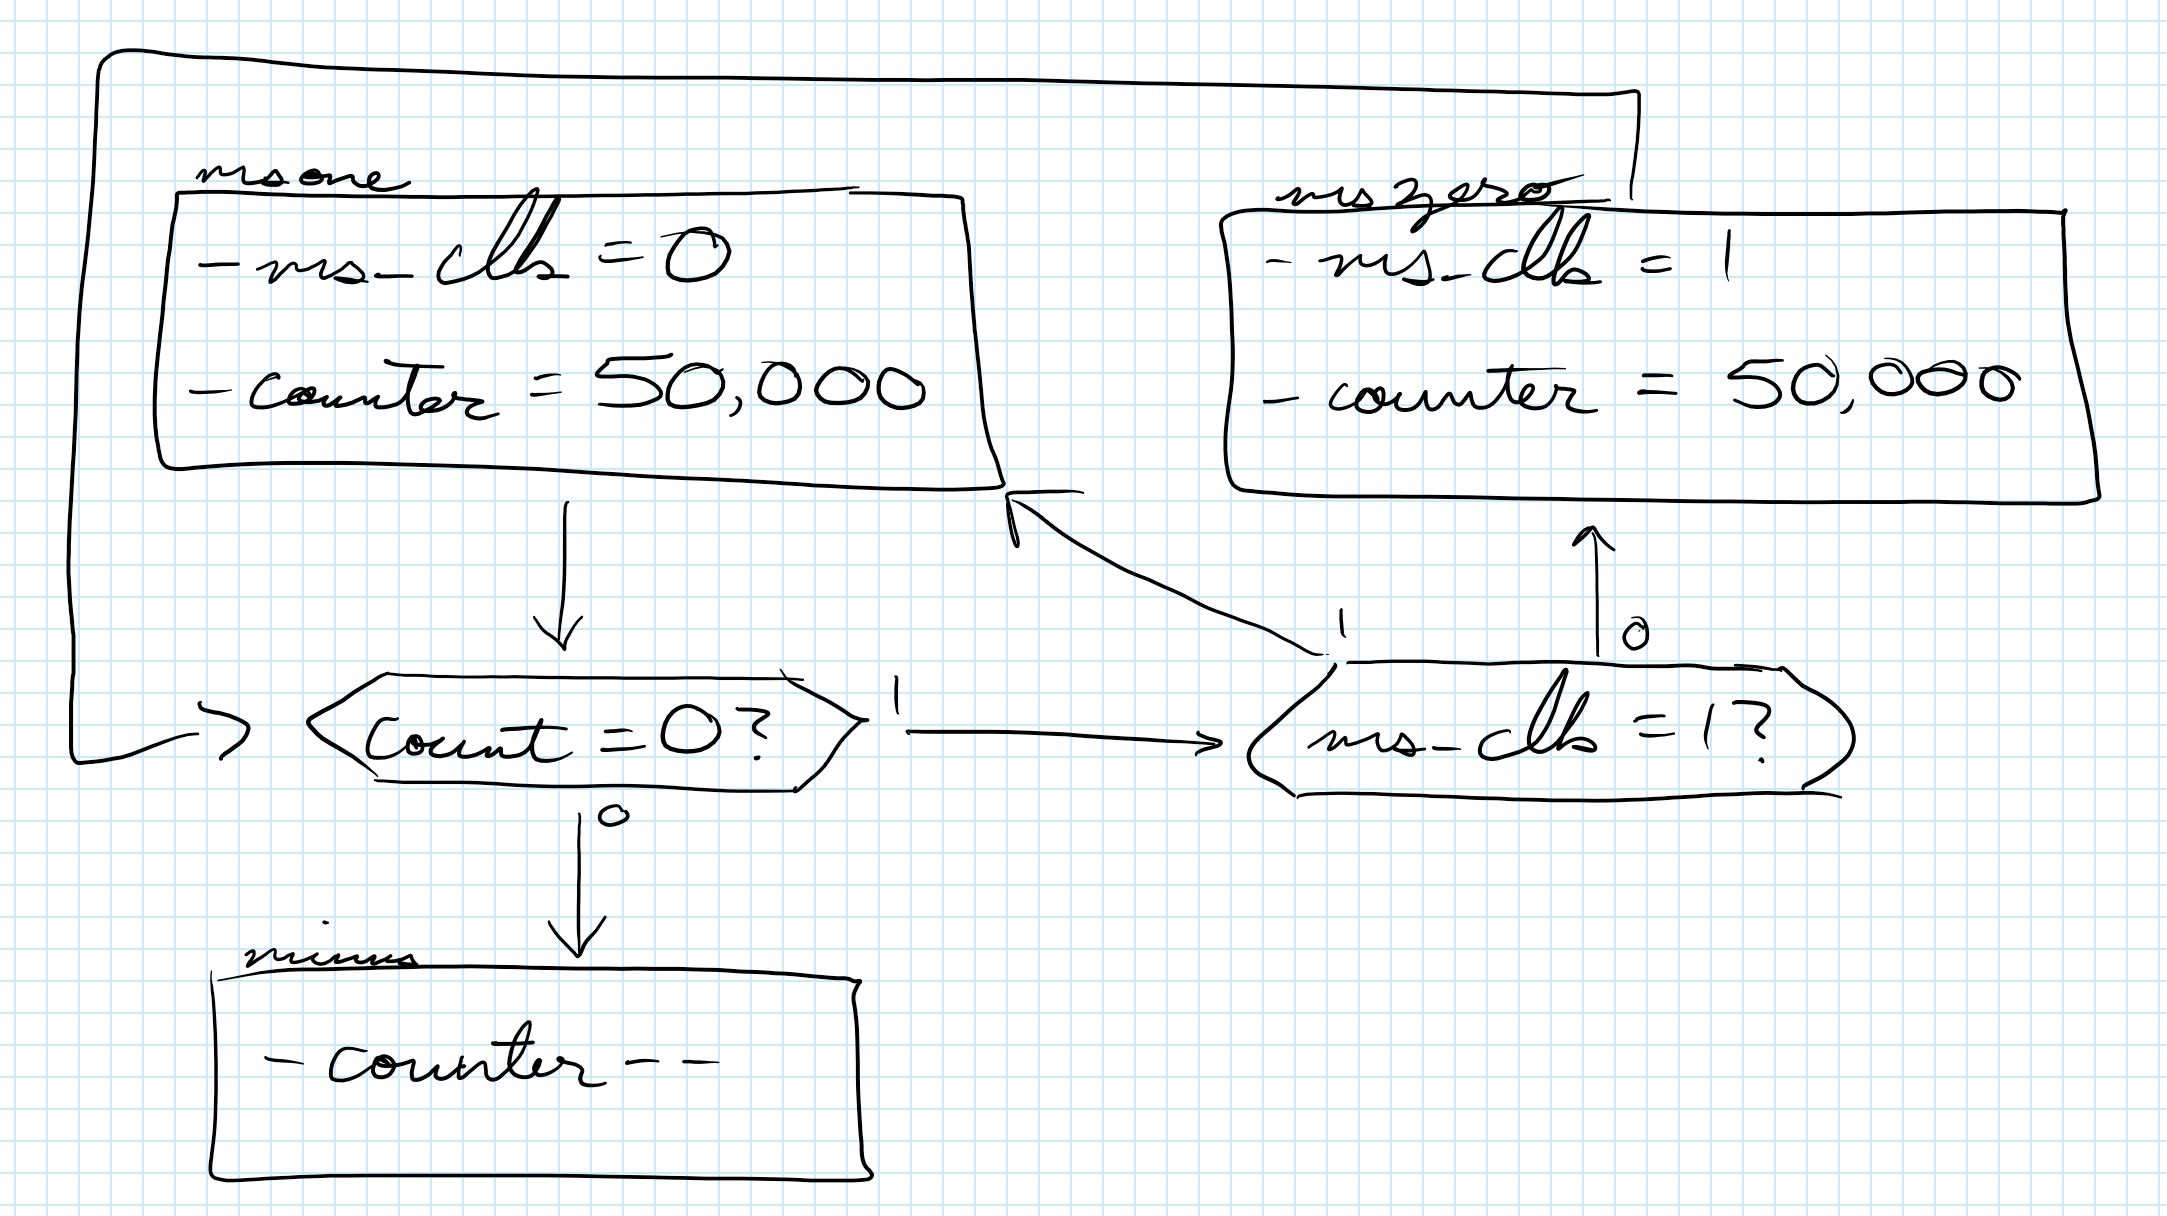
\includegraphics[width=0.9\textwidth]{ClockDividerStateMachine.jpg}
\end{center}
\end{figure}

\section{Analysis}
For readability sake, the code for this project is listed in the Appendix. Listing 1 in the Appendix shows the top level module that operates as the timer fsm. The necessary inputs and outputs that the user will need are the same in the top level module as in the board's constraint file. It is worth noting that the timer's main state machine sends simple signals to the seven-segment display mux when a simple message is to be displayed. This was added to easily change the seven-segment display in the top module. In Listing 2 in the Appendix, the clock divider is shown. This module also uses a state machine to alternate the ms\_clk bit every half of a millisecond to output a millisecond clock. Listing 3 in the Appendix shows the code for the random number generator. The output of this module is used to change the timing of the visual stimulus so that the user cannot anticipate the lighting of the LED. Listing 4 shows the code for the display mux, and Listing 5 shows the code that converts hexidecimal to seven-segment display values. Lastly, Listing 6 shows the constraints file used for the Nexys 4 DDR.  

\section{Conclusion}
The use of state machines in projects such as this one makes interacting with devices much easier. The alternative would likely be a vast number of if-statement muxes which could slow the desired output. While it would still work in this case, timing critical projects are better served using state machines. 

\section{Appendix}

\Verilog{System Verilog code for the timer state machine top module}{code:timersm}{state_machine.sv} 

\Verilog{System Verilog code for the clock divider state machine}{code:cdsm}{clock_divider.sv} 

\Verilog{System Verilog code for the random number generator}{code:rng}{fibonacci.sv} 

\Verilog{System Verilog code for the seven-segment display mux}{code:disp}{ch04_15_disp_mux.sv} 

\Verilog{System Verilog code for the hexidecimal to seven-segment converter}{code:hex}{list_ch03_14_hex_to_sseg.sv} 

\Verilog{System Verilog code for the Nexys 4 DDR constraints}{code:constraint}{Nexys4_DDR_chu.xdc} 
\end{document} 